
\chapter{METODE PENENILITIAN}


\section{Tahapan Penelitian}
Tahapan dalam penelitian ini dapat dilihat pada gambar \ref{fig:penelitian-flowchart}.
\begin{afigure}
    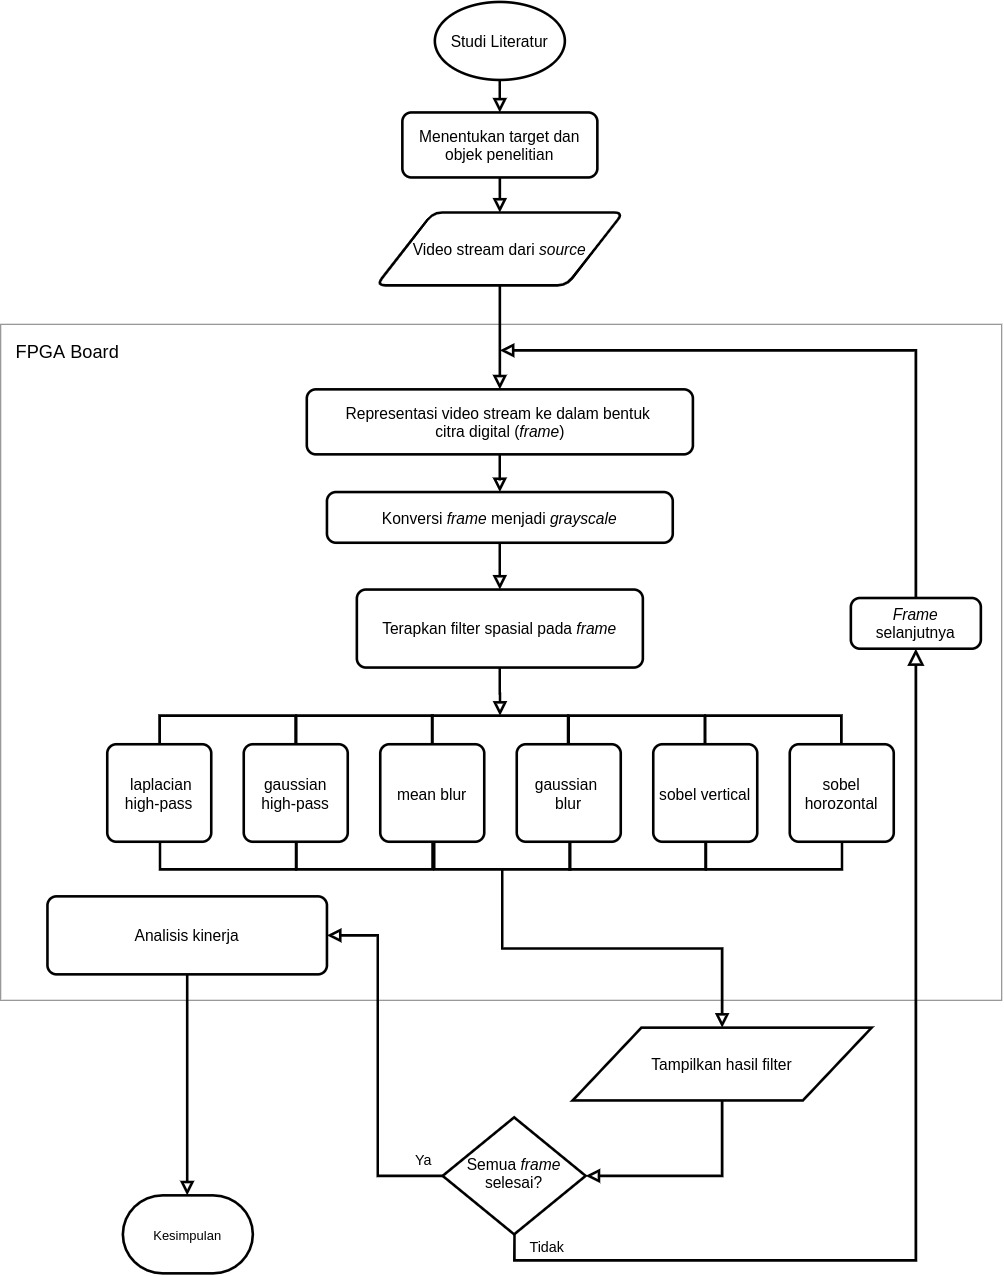
\includegraphics[width=13cm, center]{images/penelitian-flowchart.jpg}
    \caption{Flowchart tahapan penelitian.}
    \label{fig:penelitian-flowchart}
\end{afigure}
% tambahkan penjelasan lagi


\section{Waktu dan Lokasi Penelitian}
Penelitian ini dilaksanakan dari bulan Juni 2020 sampai dengan bulan Agustus 2020. Lokasi penelitian dilakukan di Laboratorium Rekayasa Perangkat Lunak Fakultas Matematika dan Ilmu Pengetahuan Alam, Universitas Hasanuddin Makassar.

\section{Rancangan Sistem}
Pada penelitian ini akan dibangun suatu sistem untuk mengimplementasikan filter spasial linear pada FPGA, dapat dilihat pada gambar \ref{fig:rancangan-sistem}.
\begin{afigure}
    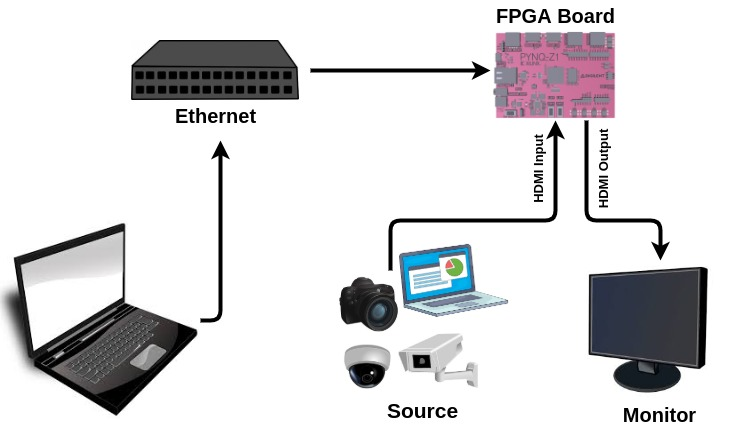
\includegraphics[width=0.85\textwidth, center]{images/rancangan-sistem.jpg}
    \caption{Rancangan sistem.}
    \label{fig:rancangan-sistem}
\end{afigure}

Video stream dari \textit{source} akan disalurkan melalui port HDMI Input pada FPGA Board, kemudian video stream tersebut akan diolah dengan menerapkan filter spasial linear pada setiap framenya. Setiap frame yang telah dilakukan filter spasial akan dialirkan ke monitor untuk kemudian ditampilkan. Kemudian dilakukan analisis kinerja pada FPGA. FPGA board yang digunakan dalam penelitian ini dapat diakses dengan \textit{ssh} pada port 22 dan dengan Jupyter Notebook melalui browser.

\section{Instrumen Penelitian}
Instrumen penelitian ini yaitu:
\begin{enumerate}[topsep=0pt,itemsep=0pt,partopsep=0pt, parsep=0pt]
    \item Kebutuhan perangkat lunak:
    \begin{enumerate}[topsep=0pt,itemsep=0pt,partopsep=0pt, parsep=0pt, label=\textbf{\alph*.}]
        \item Ubuntu 16, sebagai OS pada FPGA Board
        \item Python 3.6 (dengan modul OpenCV dan Numpy)
        \item Jupyter Notebook, sebagai interface untuk mengakses FPGA Board 
        % \item Chrome Browser 
    \end{enumerate}
    \item Kebutuhan perangkat keras:
    \begin{enumerate}[topsep=0pt,itemsep=0pt,partopsep=0pt, parsep=0pt, label=\textbf{\alph*.}]
        \item FPGA Board Xilinx PYNQ-Z2
        \item Micro SD Card 8Gb (sebagai media penyimpanan OS pada FPGA Board)
        \item Monitor Eksternal (untuk menampilkan hasil filter dari FPGA)
        \item Laptop Lenovo Ideapad 320 (sebagai source video stream)
        \item 2 buah kabel HDMI (untuk HDMI input dan HDMI output pada FPGA) 
    \end{enumerate}
\end{enumerate}
